\documentclass{article}
%\documentclass[doc,english]{apa}
\usepackage[utf8]{inputenc}

% packages
\usepackage{amsmath,amsfonts,amssymb, bm}
\usepackage{graphicx,verbatimbox}
\usepackage[colorlinks=true, allcolors=blue]{hyperref}
\usepackage{apacite}
\usepackage{authblk}  % for authors
\usepackage{caption}
%\usepackage{setspace} % doublespacing
\usepackage{subcaption}
\usepackage{booktabs}
\usepackage{nicefrac}

\usepackage{color}
\usepackage{todonotes}



\newcommand{\EJ}[1]  {\todo[inline, color=green]{EJ: {#1}}}
\newcommand{\DON}[1] {\todo[inline, color=white]{Don: {#1}}}
\newcommand{\DONa}[1]{\todo[        color=white]{Don: {#1}}}

\newcommand{\Irater}{r}
\newcommand{\Iitem}{i}
\newcommand{\Ipatient}{p}
\newcommand{\Incat}{c}
\newcommand{\Ilatent}{l}

\newcommand{\Trater}{\expandafter\MakeUppercase\expandafter{\Irater}}
\newcommand{\Titem}{\expandafter\MakeUppercase\expandafter{\Iitem}}
\newcommand{\Tpatient}{\expandafter\MakeUppercase\expandafter{\Ipatient}}
\newcommand{\Tncat}{\expandafter\MakeUppercase\expandafter{\Incat}}
\newcommand{\Tlatent}{\expandafter\MakeUppercase\expandafter{\Ilatent}}

\newcommand{\ilogit}[1]{\text{logit}^{-1}\left(#1\right)}
\newcommand{\logit}[1]{\text{logit}\left(#1\right)}
\newcommand{\dnorm}[2]{\text{Normal}\left(#1,\,#2\right)}
\newcommand{\dgamma}[2]{\text{Gamma}\left(#1,\,#2\right)}

\newcommand{\code}[1]{\texttt{#1}}
%\newcommand{\dnorm}[2]{\mathcal{N}\left(#1,\,#2\right)}
%\newcommand{\dgamma}[2]{\mathcal{G}\left(#1,\,#2\right)}


\newcommand{\osflink}{\textit{osflink}}

\title{Cultural Consensus Theory for the Evaluation of Patients’ Behavior in Psychiatric  Detention Centers}

\renewcommand{\thefootnote}{\fnsymbol{footnote}}
\author[1]{Don van den Bergh%
\thanks{Correspondence concerning this article should be addressed to: Don van den Bergh, University of Amsterdam, Department of Psychological Methods, Nieuwe Achtergracht 129, 1001 NK Amsterdam, The Netherlands. E-Mail should be sent to: donvdbergh@hotmail.com. This work was supported in part by a Research Talent grant from the Netherlands Organization of Scientic Research (NWO) awarded to EJW (???).
}}
%\author[1]{wie nog meer?}
\author[2]{Stefan Bogaerts}
\author[3]{Marinus Spreen}
\author[4]{Rob Flohr}
\author[5]{Joachim Vandekerckhove}
\author[6]{Mijke Rhemtulla}
\author[5]{William Batchelder}
\author[1]{Eric-Jan Wagenmakers}
\affil[1]{University of Amsterdam}
\affil[2]{University of Tilburg}
\affil[3]{Mesdag Clinic}
\affil[4]{Stenden University of Applied Sciences}
\affil[5]{University of California Irvine}
\affil[6]{??}
\date{}
\renewcommand*{\thefootnote}{\arabic{footnote}}
\begin{document}

\listoftodos

\noindent Dear all,

\noindent Last year, I took over Ravi Selker's project on ``A Bayesian Approach to Mental Health Assessment in Psychiatric Detention Centers''. I am writing you since you were listed in the grant proposal under collaborators. Please let me know if you are still interested in collaborating on this topic. \\

\noindent Right now I am writing the a paper on cultural consensus theory which I intend to submit for the special issue in honor of William Batchelder. If you are interested, I would appreciate it if you could provide me with feedback on the current manuscript.\\
I hope to hear from you soon.\\

\noindent Kind regards,\\
Don van den Bergh

\newpage

\maketitle

\begin{abstract}
In many psychiatric detention centers, patients' mental health is monitored at regular intervals. Typically, clinicians score patients using a Likert scale on multiple criteria including hostility. Having an overview of patients’ scores benefits staff members in at least three ways. First, the scores may help adjust treatment to the individual patient; second, the change in scores over time allow an assessment of treatment effectiveness; third, the scores may warn staff that particular patients are at high risk of turning violent. Practical importance notwithstanding, current practices for the analysis of mental health scores are suboptimal: evaluations from different clinicians are averaged (as if the Likert scale were linear and the clinicians identical), and patients are analyzed in isolation (as if they were independent). Uncertainty estimates of the resulting score are often ignored. Here we outline a quantitative program for the analysis of mental health scores using cultural consensus theory (CCT; \citeNP{Anders2015cultural}). CCT models take into account the ordinal nature of the Likert scale, the individual differences among clinicians, and the possible commonalities between patients. In a simulation, we compare the predictive performance of the CCT model to the current practice of aggregating raw observations and, as a more reasonable alternative, against often-used machine learning toolboxes. In addition, we outline the substantive conclusions afforded by application of the CCT model. We end with recommendations for clinical practitioners who wish to apply CCT in their own work. 
\end{abstract}

%\newpage

% Introduction

Psychiatric detention centers monitor the mental health of their patients at regular intervals. A clinician, psychiatrist, or another staff member, henceforth a \textit{rater}, scores a patient on multiple criteria. For example, a rater evaluates a patient's behavior on a variety of criteria that relate to aggressiveness. Next, these ratings of patients' mental health are used for multiple purposes. For instance, the scores may help adjust treatment to individual patients; second, the change in scores over time allows for an assessment of treatment effectiveness; third, the scores may warn staff that particular patients are at high risk of turning violent. Moreover, these ratings are key for a quantitative approach to monitoring and forecasting patients' behavior.

Current practices for aggregating the scores are suboptimal. Evaluations from different raters are averaged as if they are exchangeable. For example, personal communication with the staff of a psychiatric detention center suggested that clinicians are more lenient in their ratings than psychiatrists, but this information is not used to weigh their ratings. Furthermore, different patients are analyzed in isolation, as if they are independent. Any information regarding a patient's criminal offense is not accounted for in a model-based manner. In addition, any uncertainty estimates of the resulting score are usually ignored. \DON{quote opzoeken over non exchangeability van raters/ items.}

The goal of a model appropriate for these data should be to disentangle the patient, rater, and item-specific components in the data. Such a model would benefit decision making because it separates these three different sources of variances and thus decisions can be based on estimates corrected for measurement error. For example, such a model should yield estimates for a patient's aggressiveness, while accounting for rater bias, item-specific measurement error, and a patient's criminal offense. An ideal modeling framework for this is Bayesian hierarchical modeling \cite{ShiffrinEtAl2008}. In particular, Cultural Consensus Theory (CCT), which is designed to pool information from different raters and items, could be seen as a model that accomplishes exactly this -- but for a single patient. \cite{romney1986culture, batchelder1988test, batchelder2012cultural}.
%CCT models describe raters and items using hierarchical structures and thereby accommodates their individual differences. A model based on CCT would allow psychiatric detention centers to assess the effectiveness of their treatments and the mental health of their patients.
%\DON{Iets over goals en benefits!}

Here, we outline a quantitative program for the analysis of mental health scores using CCT. First, a CCT model for ordinal data is introduced \cite{Anders2015cultural}. Afterward, this model is expanded step by step, in order to include more characteristics of the data. We showcase the model in three simulation studies. First, we show that model parameters are retrieved accurately. Second, we demonstrate how CCT could be used to monitor patients progress over time. Third, we compare the predictive performance of the CCT model to the current practice of aggregating raw observations and, as a more reasonable alternative, against often-used machine learning toolboxes such as Random Forest \cite{breiman2001random} and Boosted Regression Trees \cite{friedman2002stochastic}. We showcase the substantive conclusions obtained from applying the CCT model and conclude the paper with recommendations for clinical practitioners who wish to apply CCT in their work.

\section*{Cultural Consensus Theory}
The next sections introduce Cultural Consensus Theory (CCT). First, a brief introduction to CCT is given. Afterward, the CCT model developed in \citeA{Anders2015cultural} is introduced, which serves as the simplest model for a single patient. Subsequently, this model is expanded in three steps. First, the model is expanded to describe multiple patients. Next, latent constructs are added to the model. Finally, the model is modified to include patient and rater characteristics.

Cultural Consensus Theory, also known as ``test theory without an answer key'' \cite{batchelder1988test}, is a statistical tool that attempts to retrieve the ``truth'' for an item by examining the consensus among the responses. The model accounts for varying difficulty in items and varying competence among respondents. In addition, the model can be expanded to allow for multiple consensus truths, where there may be multiple unknown truths that vary across subgroups of respondents \cite{AndersBatchelder2012}. For example, given a political questionnaire, there are no objectively correct answers. Instead, one could administer the questionnaire to left-oriented respondents and use CCT to find out what the consensus is among left oriented respondents. Rather than selecting left-oriented respondents as a target population, the questionnaire could also be given to people at random. That way, the different consensuses (e.g., left, right, center, etc.) and respondents membership to each of these could be derived from the data. The property of CCT models to estimate the consensus truth for an item from the data is ideal for psychiatric data, where a patient's true state is unknown and a consensus from the raters is desired.

The next sections formally introduce and expand the CCT models used in this paper. As a starting point, consider the Latent Truth Rater Model (LTRM), a cultural consensus model for ordinal data introduced by \citeA{Anders2015cultural}. We use a model for ordinal data as ratings are generally given on a Likert scale, but CCT can be applied to continuous data as well \cite<e.g., the LTM;>{batchelder2012cultural}. Figure~\ref{model:LTRM} shows a graphical model of the LTRM. The LTRM captures differences among raters and items and may be viewed as the simplest model for a single patient.
\begin{figure}[!ht]
%	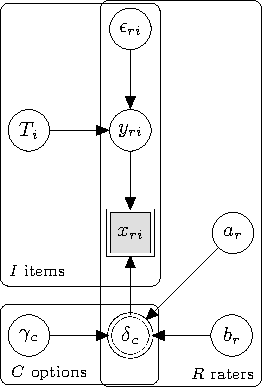
\includegraphics[width=.4\textwidth, page=1]{graphicalModels/graphicalModels.pdf}
	\begin{minipage}{0.5\textwidth}
		\centering
		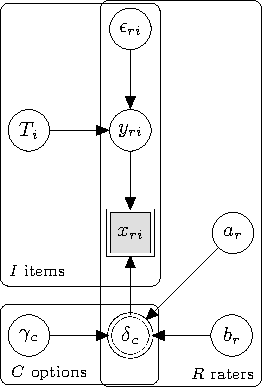
\includegraphics[width=\textwidth, page=1]{graphicalModels/graphicalModels.pdf}
		\end{minipage}\hfill
	\begin{minipage}{0.5\textwidth}
		\DON{Hierarchische componenten missen}
		{\large
		\begin{align*}
			x_{\Irater\Iitem} &\leftarrow 
			\begin{cases}
			1		&\hspace{-.3cm} \text{if } y_{\Irater\Iitem} \leq \delta_{\Irater 1} \\
			\Incat	&\hspace{-.3cm} \text{if } \delta_{\Irater, \Incat-1} < y_{\Irater\Iitem} \leq \delta_{\Irater\Incat} \\
			\Tncat	&\hspace{-.3cm} \text{if } y_{\Irater\Iitem} > \delta_{\Irater, \Tncat-1}
			\end{cases}\\
%			x_{\Irater\Iitem} &\sim OL(y_{\Irater\Iitem}, \delta_{\Irater\Incat})\\
			y_{\Irater\Iitem} &\leftarrow T_\Iitem + \epsilon_{\Irater\Iitem}\\
			\gamma_\Incat &\leftarrow \logit{\Incat / \Tncat}\\
			\delta_{\Irater\Incat} &\leftarrow a_\Irater  \gamma_\Incat + b_\Irater\\
			\sigma^\epsilon_{\Irater\Iitem} &\leftarrow \kappa_\Irater / \zeta_\Irater\\
			\sigma^\epsilon_{\Irater\Iitem} &\leftarrow \kappa_\Irater / \zeta_\Irater\\
			\epsilon_{\Irater\Iitem} &\sim \dnorm{0}{\sigma^\epsilon_{\Irater\Iitem}} \\
			T_\Iitem &\sim \dnorm{0}{10}\\
%			\zeta_\Irater   &\sim \dgamma{0.01}{0.01} \\
			\kappa_\Iitem &\sim \dgamma{0.01}{0.01} \\
			a_\Irater   &\sim \dgamma{0.01}{0.01} \\
			b_\Irater   &\sim \dnorm{0}{10}
		\end{align*}
		}%
	\end{minipage}
	\caption{Graphical model corresponding to the LTRM; a CCT model for a single patient. Gray nodes are observed whereas white nodes are unobserved parameters. Square nodes are discrete and circular nodes are continuous. A double border implies that a node is ???.}
	\label{model:LTRM}
\end{figure}
\DON{Definieer Ordered Logistic als een kansverdeling met locatie, scale en thresholds als parameters.}
The rating given by rater $\Irater$ on item $\Iitem$ is denoted $x_{\Irater\Iitem}$ and takes on discrete values from $1$ through $\Tncat$. \citeA{Anders2015cultural} formalize the core ideas of the LTRM with 6 axioms. There is a latent, shared cultural truth among the raters, which is captured by the item location parameters $T_\Iitem$ (Axiom 1). Since raters are not perfect measurement instruments, they infer a noisy version of the cultural truth for each item, called a latent appraisal and defined as $y_{\Irater\Iitem} = T_\Iitem + \epsilon_{\Irater\Iitem}$, where $\epsilon_{\Irater\Iitem}\sim \dnorm{0}{\sigma^\epsilon_{\Irater\Iitem}}$ (Axiom 2). The standard deviation of the appraisal error $\sigma^\epsilon_{\Irater\Iitem}$ reflects that raters differ in their precision, captured by $\zeta_\Irater$, and that items differ in their difficulty, captured by $\lambda_\Irater$. These two components define the standard deviation, $\sigma^\epsilon_{\Irater\Iitem} = \kappa_\Irater / \zeta_\Irater$ (Axiom 3). Latent appraisals are assumed to be conditionally independent given the latent truth $T_\Iitem$ and the appraisal error $\epsilon_{\Irater\Iitem}$ (Axiom 4). So far, the axioms describe a latent process that underlies each observation. To translate these latent appraisals to observed categorical responses, it is assumed that there exist $\Tncat - 1$ ordered thresholds $\delta_{\Irater\Incat}$, such that each $x_{\Irater\Iitem}$ is generated in the following way (Axiom 5):
\begin{align*}
	x_{\Irater\Iitem} = 
	\left\{\begin{array}{ll} 
	1		& \text{if } y_{\Irater\Iitem} \leq \delta_{\Irater 1} \\[4pt]
	\Incat	& \text{if } \delta_{\Irater, \Incat-1} < y_{\Irater\Iitem} \leq \delta_{\Irater\Incat} \\[4pt]
	\Tncat	& \text{if } y_{\Irater\Iitem} > \delta_{\Irater, \Tncat-1}
	\end{array} \right.
\end{align*}
In practice, the generating process of $x_{\Irater\Iitem}$ is probabilistic and described with an ordered logistic distribution\footnote{The choice for an ordered logistic distribution is arbitrary and an ordered probit distribution could also be used, as was done by \citeA{Anders2015cultural}.}, which gives:
\begin{align*}
P(x_{\Irater\Iitem}\mid y_{\Irater\Iitem},\delta_{\Irater}) = 
\left\{\begin{array}{ll} 
1 - \ilogit{y_{\Irater\Iitem} - \delta_{\Irater 1}}         & \text{if } x_{\Irater\Iitem} = 1, \\[4pt]
\ilogit{y_{\Irater\Iitem} - \delta_{\Irater,\Incat-1}} - 
\ilogit{y_{\Irater\Iitem} - \delta_{\Irater\Incat}}         & \text{if } 1 < x_{\Irater\Iitem} < \Tncat,\\[4pt]
\ilogit{y_{\Irater\Iitem} - \delta_{\Irater,\Tncat-1}}       & \text{if } x_{\Irater\Iitem} = \Tncat. 
\end{array} \right.
\end{align*}
The thresholds $\delta_{\Irater\Incat}$ are not fixed across raters but accommodate the response biases of the raters. \citeA{Anders2015cultural} do so by estimating $\Tncat-1$ ordered thresholds $\gamma$ and defining $\delta_{\Irater\Incat} = a_\Incat \gamma_\Incat + b_\Incat$ (Axiom 6). This translation of thresholds is called the Linear in Log Odds function and is a useful tool for capturing bias in probability estimation \cite{Fox1995, Gonzalez1999, Anders2015cultural}.

A technical difficulty of estimating $\Tncat-1$ is that the number of thresholds $\gamma_\Incat$ increases with the number of response options. This introduces a large number of parameters that can be difficult to estimate, in particular when some response options are not observed (i.e., when there are ceiling or floor effects). In addition, the model is only identified if the sum of thresholds is zero ($\sum_{\Incat=1}^{\Tncat}\gamma_\Incat = 0$; otherwise adding a constant to $T_\Iitem$ and $\gamma_\Incat$ yields an identical likelihood). Rather than modeling each threshold individually, we model the thresholds as deviances from an initial guess, $\gamma_\Incat = \logit{c/C}$. This yields a set of thresholds such that if the latent appraisal is 0 then $P(x_{\Irater\Iitem})$ is uniform. Response biases are incorporated in the same manner: $\delta_{\Irater\Incat} = a_\Irater\logit{c/C} + b_\Irater$. This simplification can still capture a wide variety of data sets \cite{Selker2019}.

Figure~\ref{fig:orderedLogistic} provides an intuition for how the ordered logistic distribution can model different data sets. In the left panel, there is no response bias, $a_\Irater = 1$ and $b_\Irater = 0$, which yields a uniform distribution over the outcomes. In the right panel, an increase in response scale, $a_\Irater = 2$, concentrates the responses around the middle outcomes. An increase in response shift, $b_\Irater = .5$ moves the average response towards lower categories. The latent appraisal is the same in both panels.
\begin{figure}[!ht]
	\centering
	\begin{subfigure}{.5\textwidth}
		\centering
		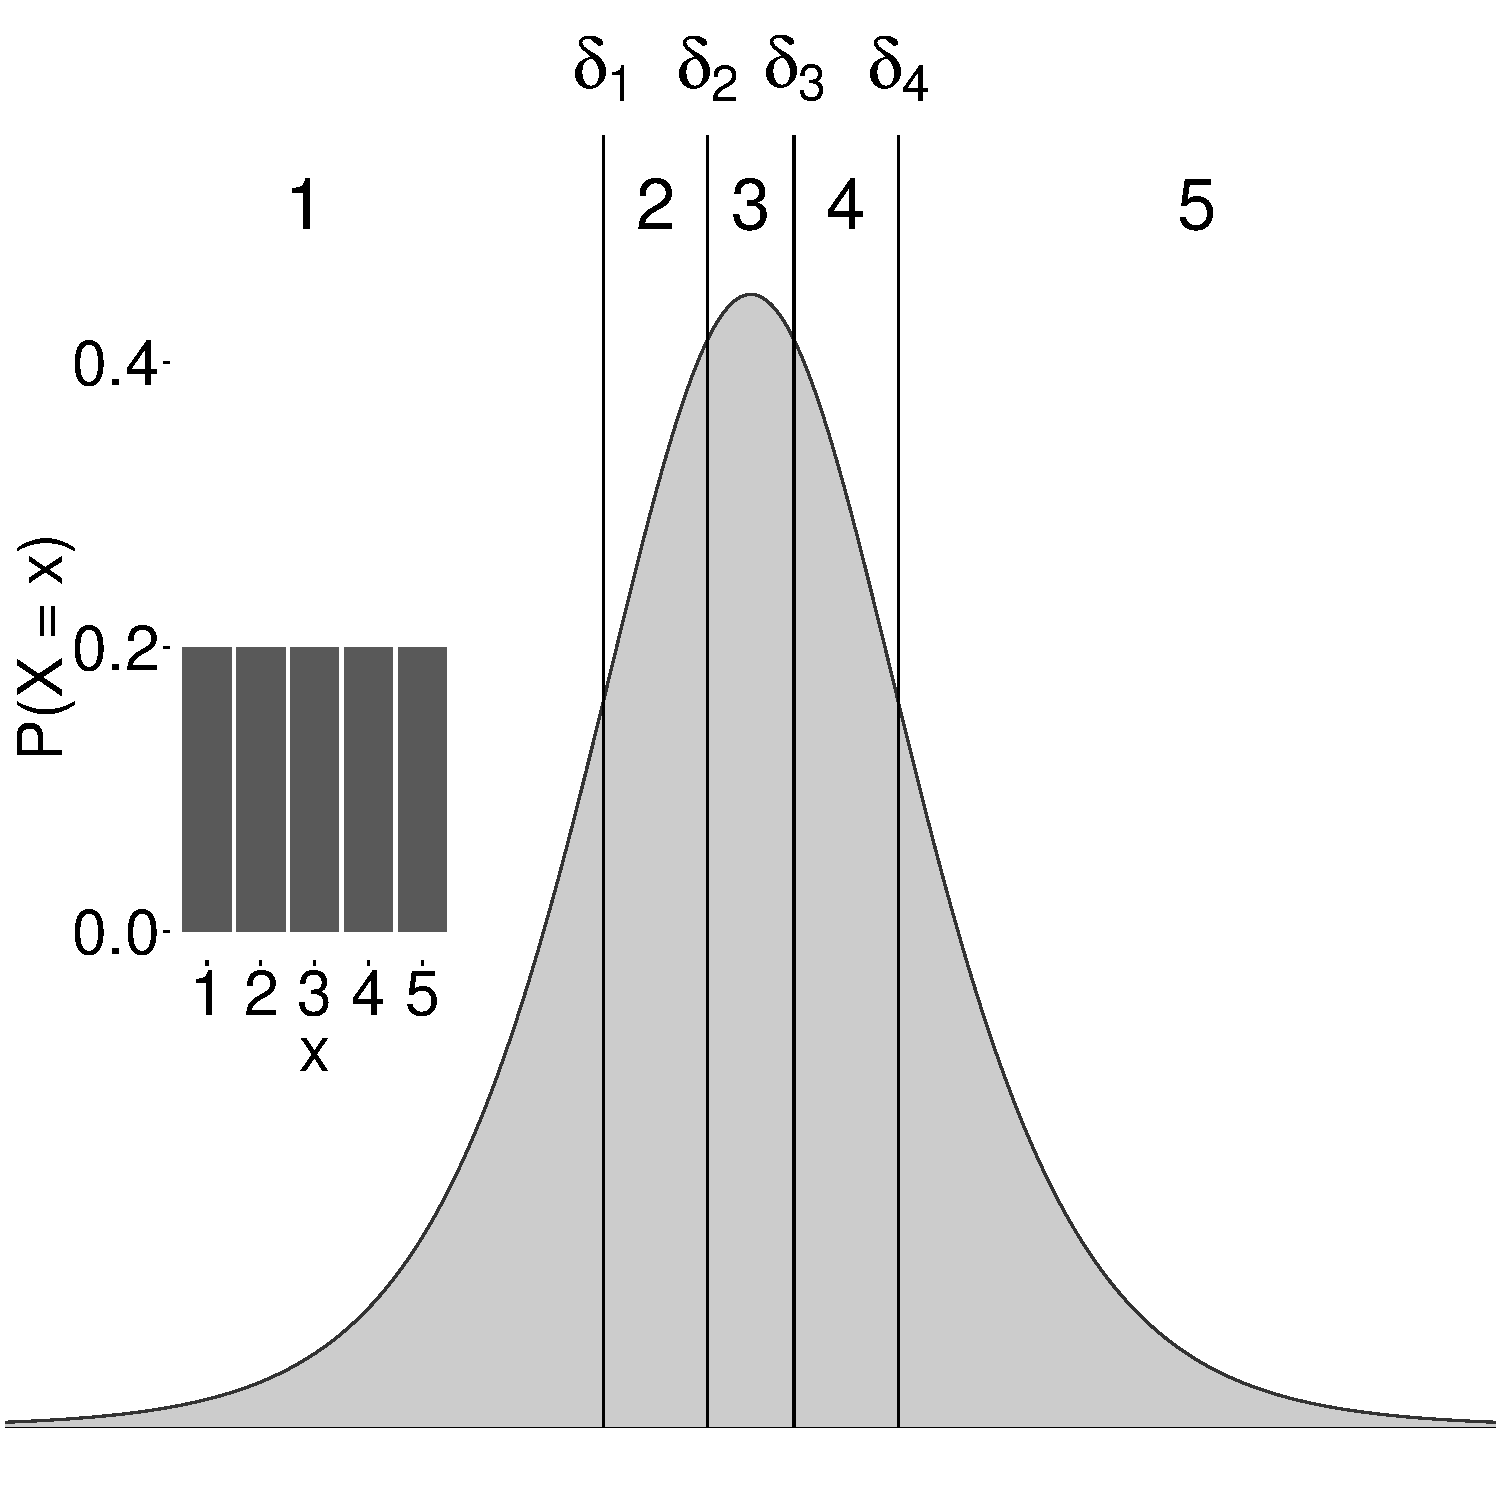
\includegraphics[width=.98\textwidth]{figures/orderedLogisticUnbiased.pdf}
%		\caption{A subfigure}
%		\label{fig:sub1}
	\end{subfigure}%
	\begin{subfigure}{.5\textwidth}
		\centering
		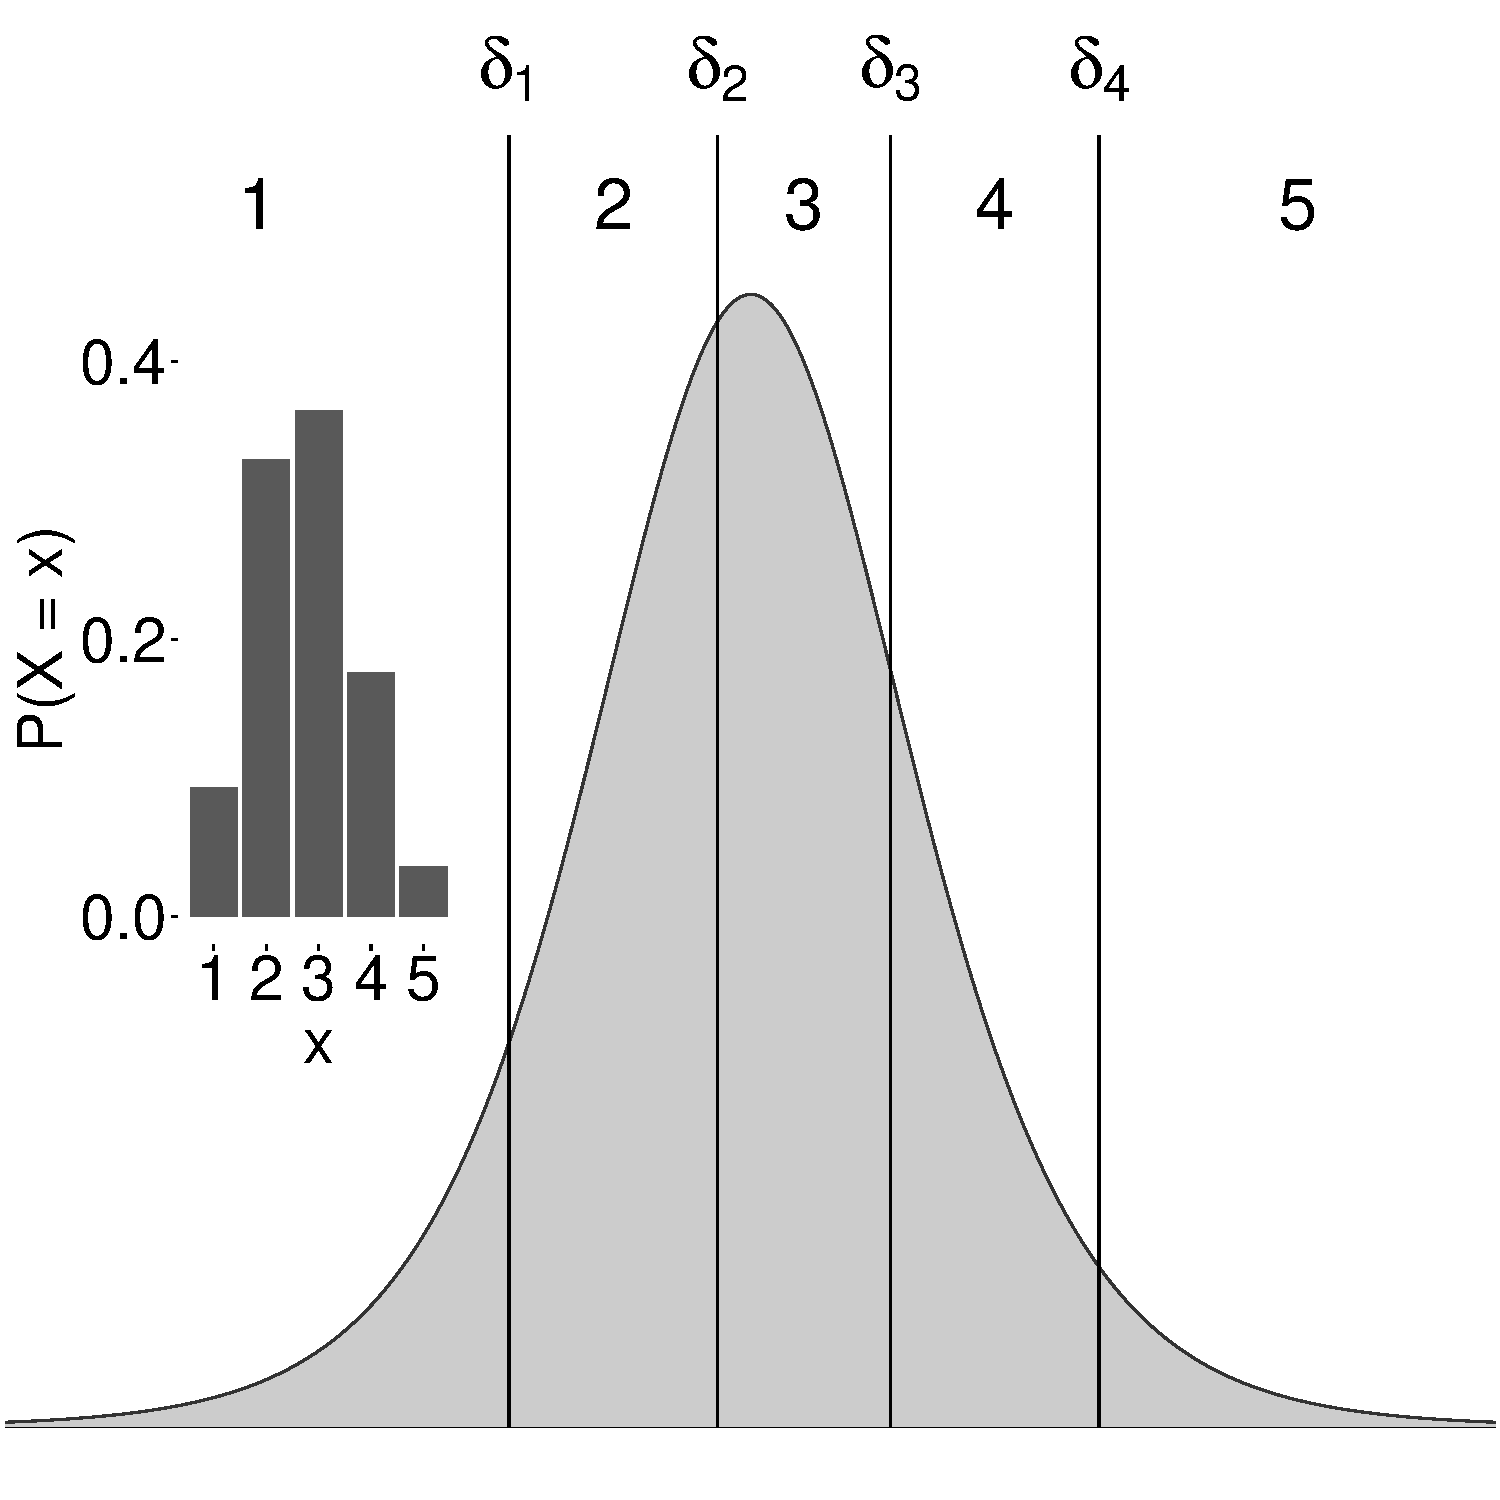
\includegraphics[width=.98\textwidth]{figures/orderedLogisticBiased.pdf}
%		\caption{A subfigure}
%		\label{fig:sub2}
	\end{subfigure}
	\caption{Ordered Logistic Distribution for $y_{\Irater\Iitem} = 0$ and varying thresholds. The implied probability distribution over categories is shown inside each panel. In the left panel, there is no response bias, $\alpha_\Irater = 1$, $\beta_\Irater = 0$. As a consequence, the distribution over outcomes is uniform. In the right panel, the thresholds are shifted right and the scale increased slightly, $\alpha_\Irater = 2$, $\beta_\Irater = 0.5$. The distribution over outcomes is peaked on 2 and 3.}
	\label{fig:orderedLogistic}
\end{figure}

The first extension is to allow the model to describe multiple patients. This can be achieved by allowing all item specific parameters to vary across patients ($T_{\Iitem\Ipatient}, \kappa_{\Iitem\Ipatient}$, which induces $\epsilon_{\Irater\Iitem\Ipatient}, y_{\Irater\Iitem\Ipatient}, x_{\Irater\Iitem\Ipatient}$). This implies that the latent cultural truth of an item and the difficulty of an item vary across patients. A second extension is that we are often not just interested in the latent truth of a single item, but also in a construct that is measured by multiple items. This is essentially a factor model, where a latent construct (e.g., aggressiveness) is measured through multiple items. For this particular application, however, the items may contain rater bias which is simultaneously estimated and corrected for. Formally, there are $\Tlatent$ constructs captured by latent variables which are indicated by some items. The measurement model, i.e., which items load on what construct, is assumed to be known. 

%Adding these two concepts to the LTRM model results in the graphical model shown in Figure~\ref{model:LTRM2}.
%\begin{figure}[!ht]
%	\centering
%	\includegraphics[width=.6\textwidth, page=2]{graphicalModels/graphicalModels.pdf}
%	\caption{Graphical model corresponding to the CCT model for multiple patients.}
%	\label{model:LTRM2}
%\end{figure}
%\begin{figure}[!ht]
%\begin{minipage}{0.5\textwidth}
%		\centering
%		\includegraphics[width=1\textwidth, page=2]{graphicalModels/graphicalModels.pdf}
%\end{minipage}\hfill
%\begin{minipage}{0.5\textwidth}
%	{\large
%		\begin{align*}
%		T_{\Iitem\Ipatient} &\sim \dnorm{\lambda_{\Iitem\Ilatent}\eta_{\Ilatent\Ipatient}}{1}\\
%		\eta_{\Ilatent\Ipatient} &\sim \dnorm{0}{1} \\
%		\end{align*}
%	}%
%\end{minipage}
%\caption{Graphical model corresponding to the CCT model for multiple patients.}
%\label{model:LTRM2}
%\end{figure}


%\DON{Als we het delict in de prior stoppen, dan moet het zo zijn dat elke moordenaar aggressiever is dan elke kindermisbruiker, ongeacht of een moordenaar al 30 jaar vast zit. Dat is wel erg resrictief.}
A third extension is to add additional information about raters and patients to the model. This would facilitate the model to capture that, for instance, child molesters are less aggressive than murderers. Such patient and raters characteristics could be perceived as covariates and their influence could be captured through a regression. For instance, the crime of a patient can be regressed on each latent variable, allowing the model to capture that child molesters and murderers differ in aggression, but not in say ... \DONa{ik heb eigenlijk geen idee wat ze allemaal meten}. Rater characteristics could be regressed directly on the latent appraisal. Adding these three components to the model results in the graphical model shown in Figure~\ref{model:LTRM3}.

\begin{figure}[!ht]
	%	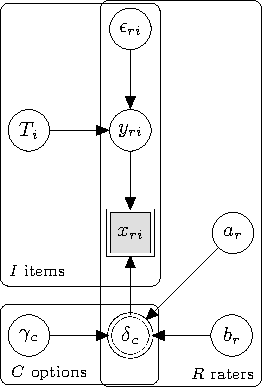
\includegraphics[width=.4\textwidth, page=1]{graphicalModels/graphicalModels.pdf}
	\begin{minipage}{0.5\textwidth}
		\centering
		\centering
		\includegraphics[width=1\textwidth, page=3]{graphicalModels/graphicalModels.pdf}
	\end{minipage}\hfill
\begin{minipage}{0.5\textwidth}
%\DON{Hierarchische componenten missen}
{\large
	\begin{align*}
%	x_{\Irater\Iitem} &\leftarrow 
%	\begin{cases}
%	1		&\hspace{-.3cm} \text{if } y_{\Irater\Iitem} \leq \delta_{\Irater 1} \\
%	\Incat	&\hspace{-.3cm} \text{if } \delta_{\Irater, \Incat-1} < y_{\Irater\Iitem} \leq \delta_{\Irater\Incat} \\
%	\Tncat	&\hspace{-.3cm} \text{if } y_{\Irater\Iitem} > \delta_{\Irater, \Tncat-1}
%	\end{cases}\\
%	y_{\Irater\Iitem} &\leftarrow T_\Iitem + \epsilon_{\Irater\Iitem}\\
%	\gamma_\Incat &\leftarrow \logit{\Incat / \Tncat}\\
%	\delta_{\Irater\Incat} &\leftarrow a_\Irater  \gamma_\Incat + b_\Irater\\
%	\sigma^\epsilon_{\Irater\Iitem} &\leftarrow \kappa_\Irater / \zeta_\Irater\\
%	\epsilon_{\Irater\Iitem} &\sim \dnorm{0}{\sigma^\epsilon_{\Irater\Iitem}} \\
	T_{\Iitem\Ipatient} &\sim \dnorm{\lambda_{\Iitem\Ilatent}\eta_{\Ilatent\Ipatient}}{1}\\
	\eta_{\Ilatent\Ipatient} &\sim \dnorm{w_{\Ipatient\Ilatent}}{10} \\
	w_{\Ipatient\Ilatent} & \sim\dnorm{0}{10} \\
	b_\Irater   &\sim \dnorm{z_\Irater}{10}\\
	z_\Irater &\sim \dnorm{0}{10}
	\end{align*}
}%
\end{minipage}
	\caption{Graphical model corresponding to the CCT model for multiple patients. Rater characteristics are captured by $z_\Irater$ and patient characteristics are captured by $w_\Ipatient$.}
	\label{model:LTRM3}
\end{figure}

\section*{Simulation Results}

The sections below illustrate the LTRM in a variety of scenarios. First, we demonstrate that the parameters of the LTRM can be accurately retrieved. Afterward, we show how the LTRM could monitor the progress of a patient across measurement occasions. Finally, we compare the predictive performance of the LTRM to the unweighted mean of the observations and two machine learning toolboxes.

In all simulations, data were simulated using R \cite{R} and the posterior distributions were approximated with variational inference using Stan \cite{CarpenterEtAl2017Stan}. We opted to use variational inference over traditional Markov chain Monte Carlo because it was computationally fast while providing similar results in terms of parameter retrieval and model predictions. Random Forest and Boosting analyses were done using the R packages \code{ranger} and \code{gbm} respectively \cite{ranger2017, gbmPackage}. The tuning parameters of the machine learning methods were optimized using the R package \code{caret} \cite{kuhn2008building}. R files and Stan models are available in the online appendix at \osflink{}.
%\DON{Fill in refs.}

\subsection*{Parameter Retrieval}
Before interpreting a model, it is key to assess if its parameters can be accurately retrieved. For this purpose, we simulated a data set of 50 patients, 30 raters, 20 items, and 5 answer categories. A patient-specific covariate containing 5 levels was added to mimic the effect of a patient's criminal offense. Similarly, three different categories of raters were assumed, which was also captured as a covariate. Parameter retrieval is shown in Figure~\ref{fig:parameterRecoveryM3}, which graphs the values used to simulate data with against the posterior mean for each parameter. 

\begin{figure}[!ht]
	\centering
	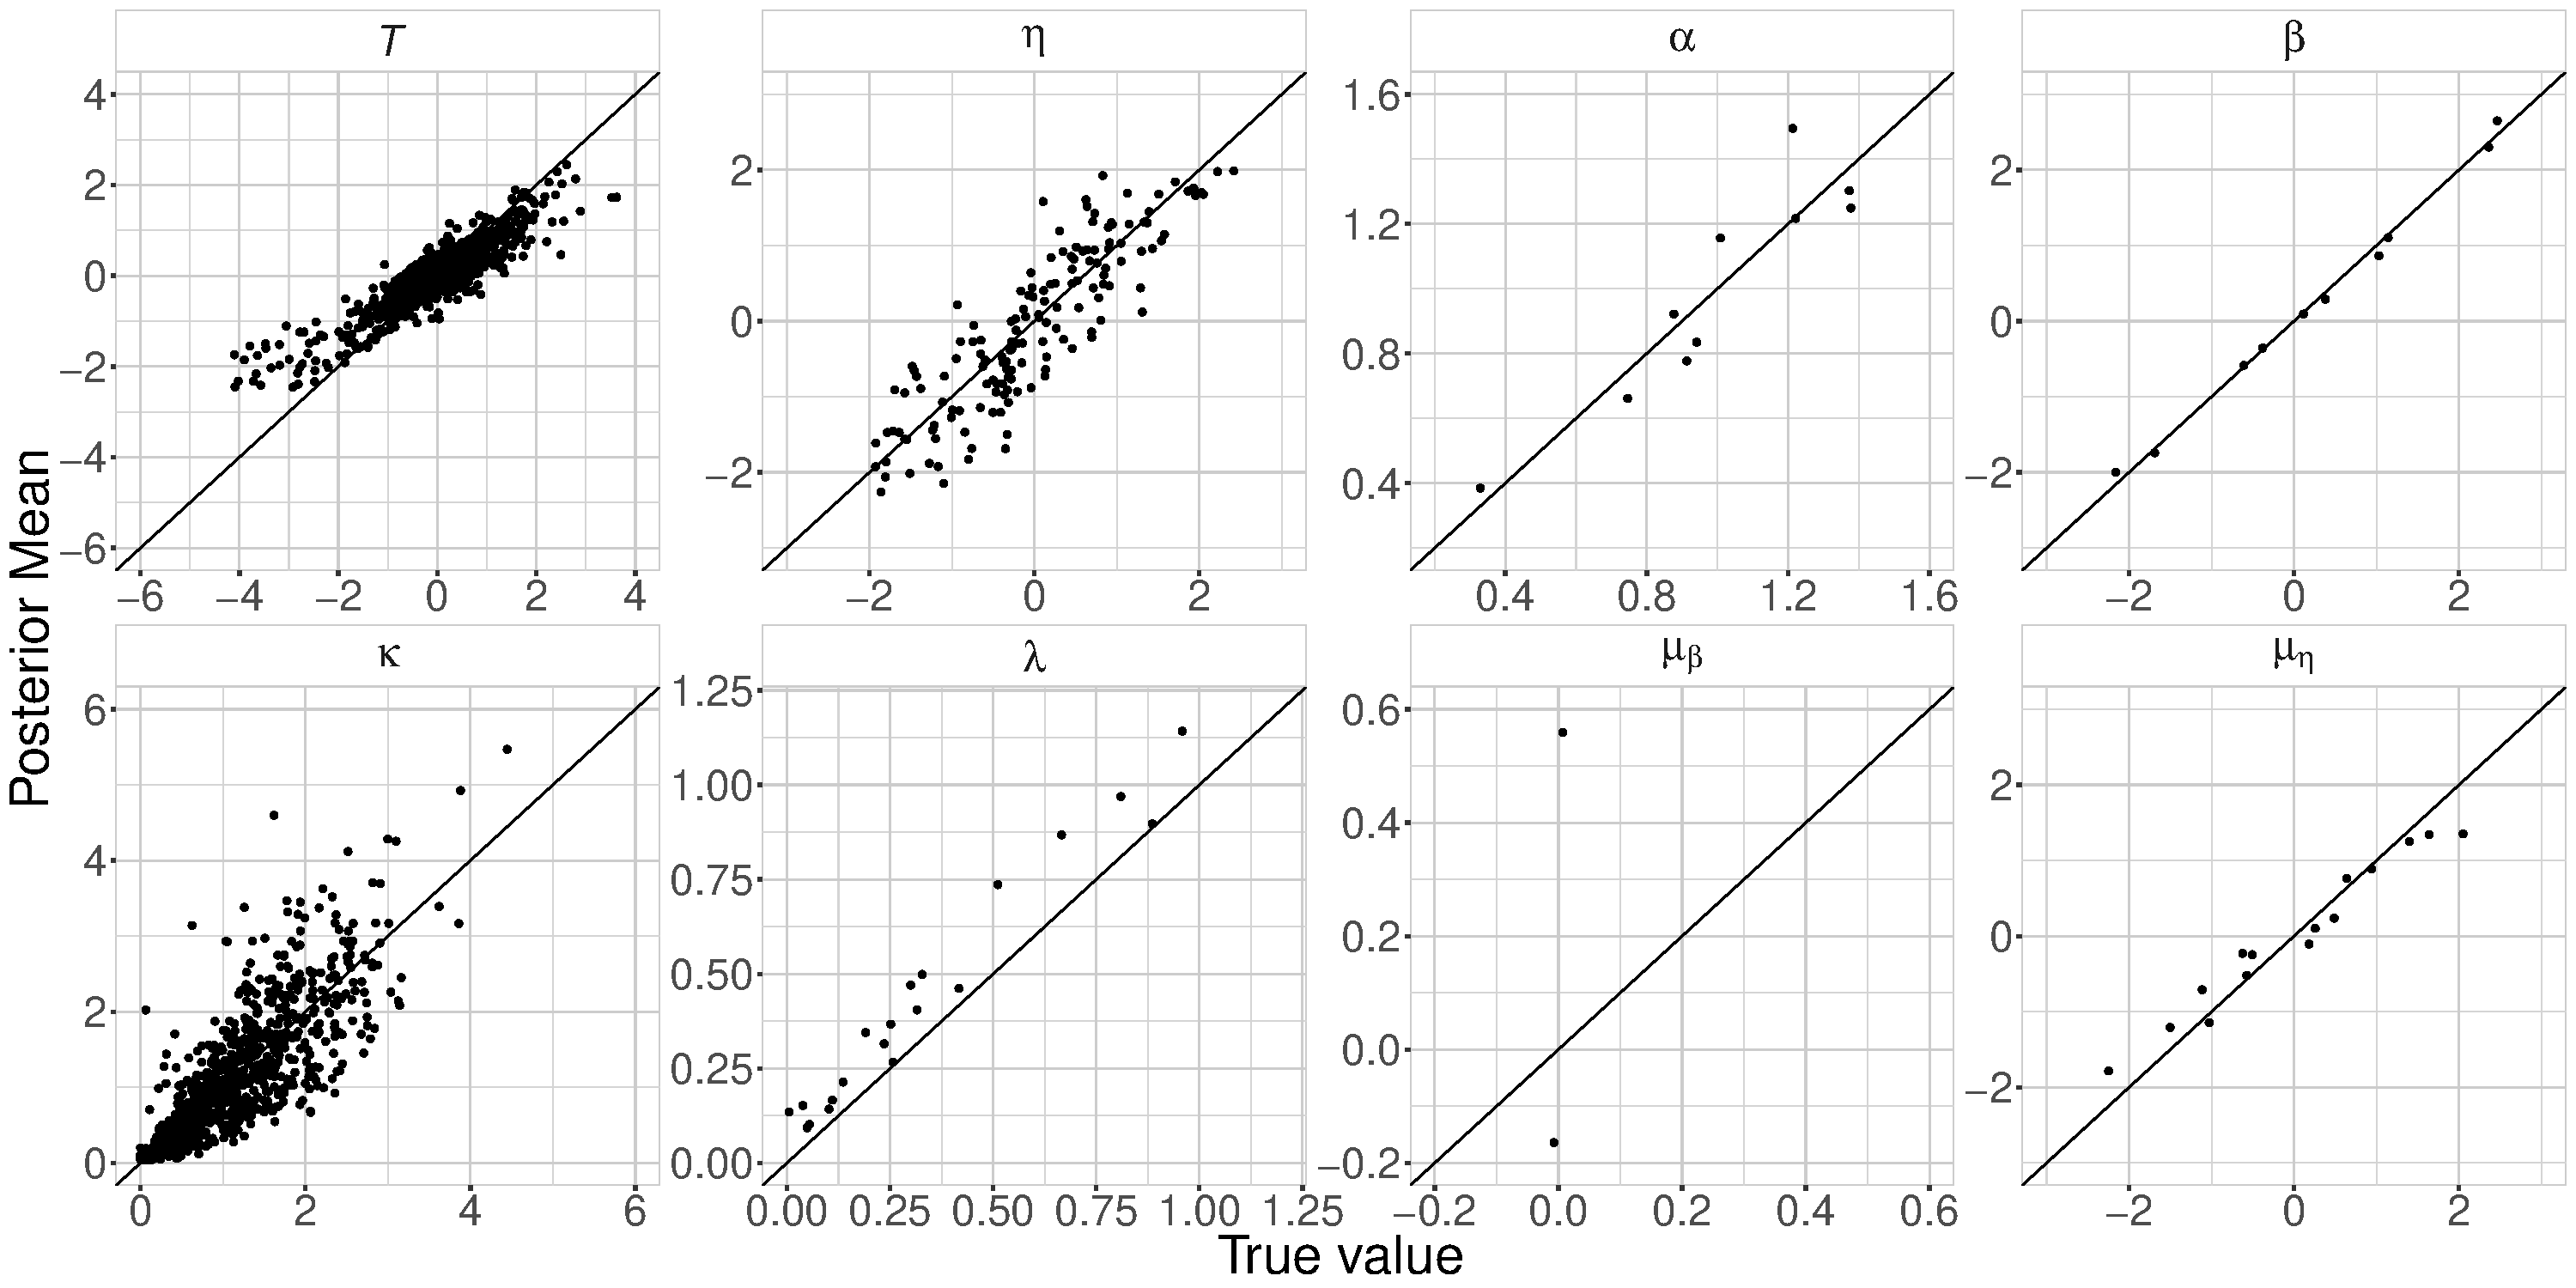
\includegraphics[width= \textwidth]{figures/parameterRecoveryModel3.pdf}
	\caption{True value used for data simulation (x-axis) and posterior mean of that parameter (y-axis), for all parameters of the LTRM. Above each panel is indicated which parameter is shown.}
	\label{fig:parameterRecoveryM3}
\end{figure}

All parameters are retrieved adequately. An exception is $\kappa$, which estimates appear more variable as the true value $\kappa$ increases. However, the spread in the posterior means of $\kappa$ is similar to that in Figure~6 of \citeA{Anders2015cultural}. Also, the posterior means of $\mu_\beta$ are approximately equal to the sample means of $\beta_\Irater$ split by the rater specific covariates. These sample means differ somewhat from the true means since there are 10 observations per mean.

\subsection*{Progress Monitoring}

Ideally, patients are monitored over a period of time and data from multiple measurement occasions is obtained. Next, the LTRM is applied to analyze the data. However, the LTRM should not be applied to data from individual measurement occasions, because an identification restriction of the LTRM is that the mean of each latent construct is zero. Instead, the LTRM can be easily expanded with an intercept that varies across patients, latent constructs, and measurement occasions. As a result, the progress for a single patient on one construct could be visualized as in Figure~\ref{fig:progressMonitoring}.

\begin{figure}[!ht]
	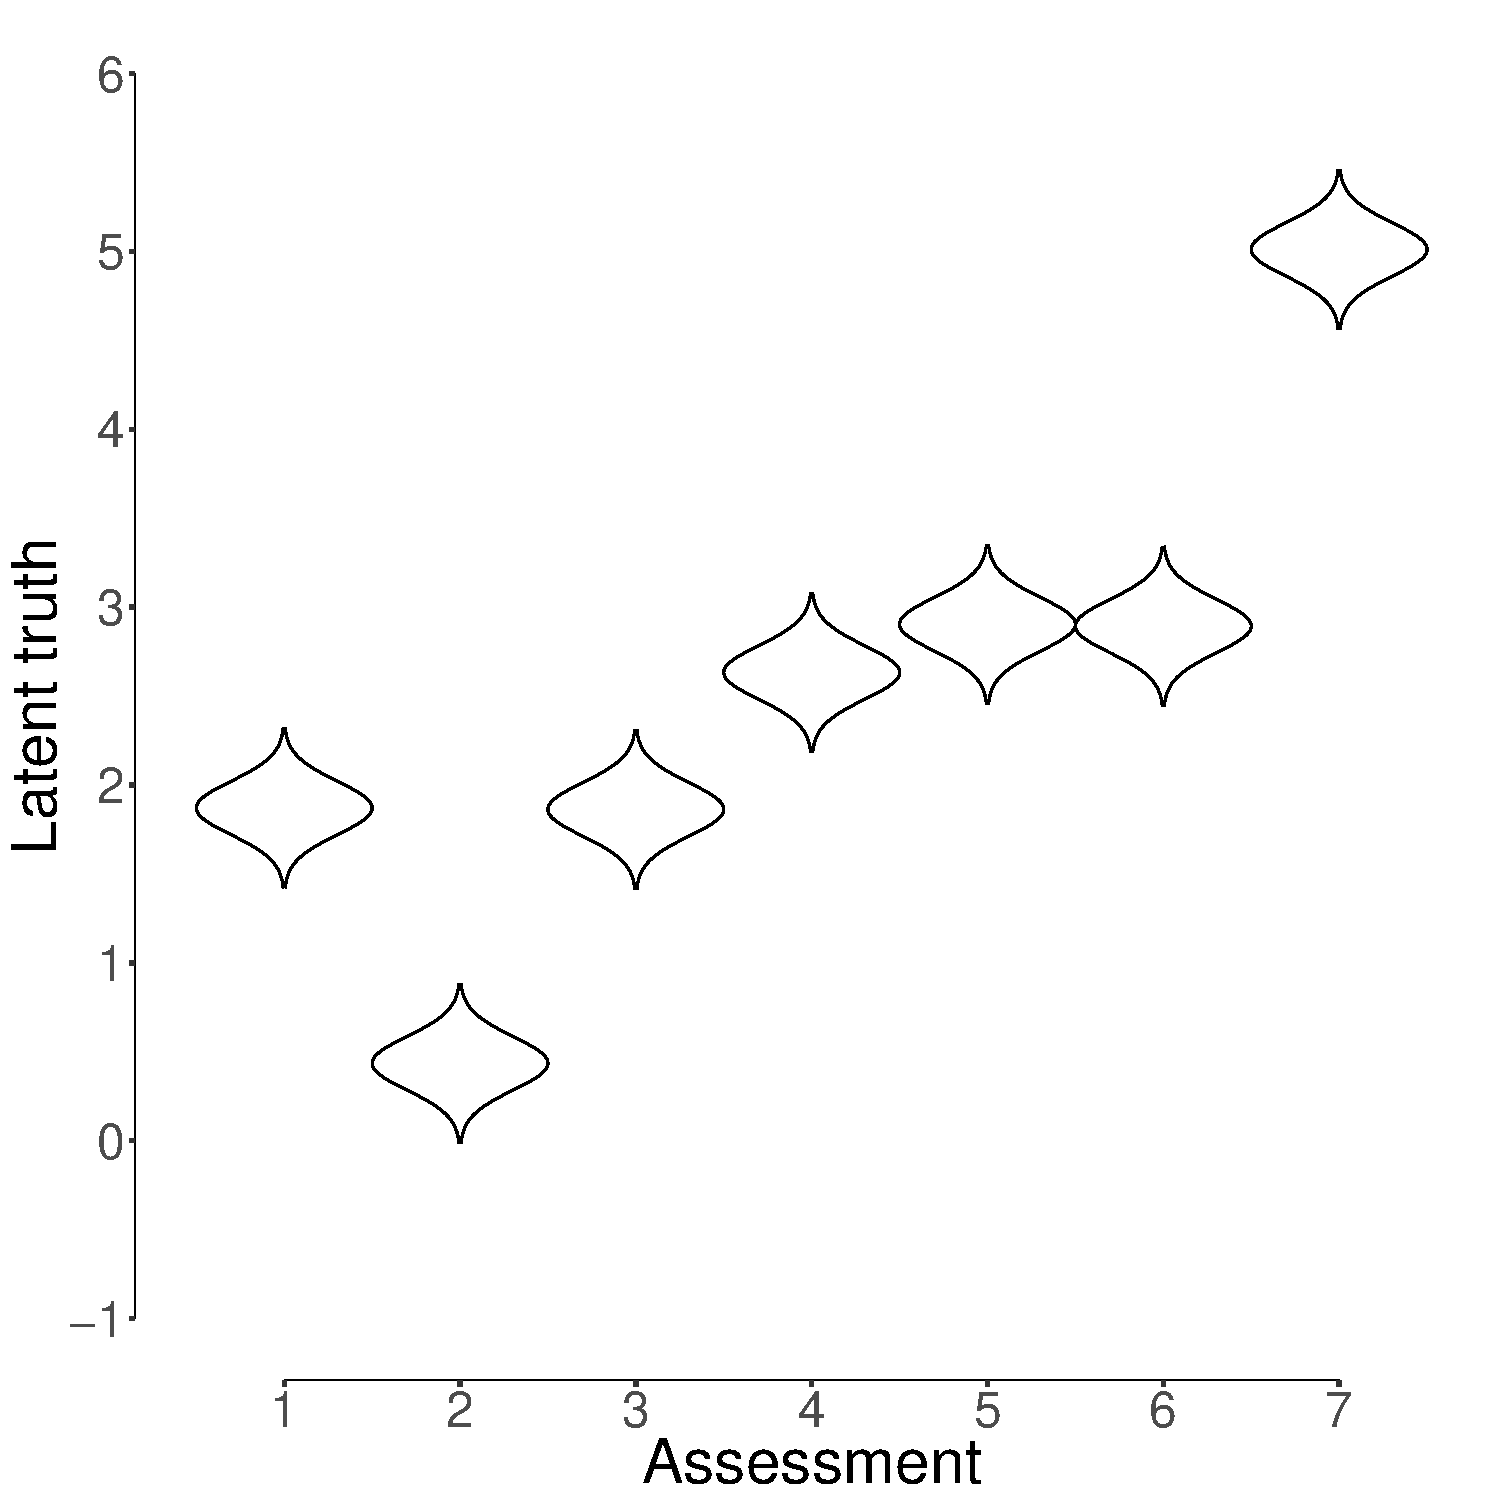
\includegraphics[width=\linewidth]{figures/progressMonitoring.pdf}
	\caption{Example of how a patient's progress on a single construct could be monitored across measurement occasions.}
	\label{fig:progressMonitoring}
\end{figure}

\subsection*{Predictive Performance}
Here, the predictive performance of the LTRM is compared to that of the mean and, as a more informative comparison, to Random Forest and Boosted Regression Trees, henceforth Boosting. 
%Consider the following scenario: Given one measurement occasion for multiple patients, the goal is to predict the behavior of those patients for the next day. It is assumed that patients remain unchanged from one day to the next, i.e., the generating model remains the same. 
We simulated a consisting of 20 raters, 25 items, 30 patients, and thus in total 15,000 observations. This data set was split into a training set (90\%) and a test set (10\%). The performance of the three methods was evaluated by training the models on the training set and using the trained model to predict the outcomes for a test set. For the LTRM, we used the mode of the posterior predictive distribution as a point-prediction\footnote{In this particular example, model predictions could also be interpreted as imputing a missing value. If these are regarded as missing observations rather than predictions, they should be modeled as unknown discrete parameters of the model \cite<Ch.~8;>{GelmanEtAl2014BDA}. That way, uncertainty about these missing observations is propagated into the parameters. Although we did not sample the missing observations from the joint posterior distribution, the code in the online appendix does show how to do this.}, whereas for Random Forest and Boosting, we used the majority vote. Rather than the commonly used mean (which predictions lie outside of the ordinal scale), we used the observed mode of all observations for the same rater, item, or patient (i.e., mode$(x_{-r,ip},x_{r,-i,p},x_{ri,-p})$).

A technical difference between this approach and the previous simulation is that model predictions are effectively treated as missing data. In terms of implementation, a complete data set, where every patient is scored on each item by all raters, is represented as an array of dimensions $\Trater\times\Titem\times\Tpatient$ (and possibly a dimension for measurement occasion). However, it is easier to handle an incomplete data set by representing the data as a matrix of $(\Trater\times\Titem\times\Tpatient)$ rows and $4$ columns (i.e., long format).\footnote{For a Stan implementation the long format is even required as missing values must be handled explicitly, unlike e.g., JAGS.} In this format, the first column indicates the outcome, the second the rater, the third the item, the fourth the patient, and subsequent columns indicate rater and patient covariates.

We quantified prediction error by calculating the confusion matrix, a frequency table of predicted versus hold-out responses where the diagonal indicates the number of correct responses. Prediction accuracy is defined as the number of correct responses divided by the total number of responses.

\begin{table}[!ht]
	\centering
	\caption{Prediction accuracy for the LTRM, Random Forest, Boosting, and the sample mode. The LTRM outperforms all other methods.}
	\begin{tabular}{lr}
		\hline
		Method & Prediction Accuracy \\ 
		\hline
		LTRM 		  & 0.52 \\ 
		Random Forest & 0.40 \\ 
		Boosting 	  & 0.35 \\ 
		Sample Mode   & 0.41 \\ 
		\hline
	\end{tabular}
\end{table}

Although Random forest and Boosting are excellent black box algorithms for prediction, with default settings these algorithms initially performed worse than the observed mode. Therefore, we optimized the hyperparameters of Random Forest and Boosting \cite{kuhn2008building}.

Given that the data were generated by the LTRM, it comes as no surprise that it predicts more accurately than the other methods. However, even though data generated from the LTRM is likely a gross simplification of reality, the results show that black box machine learning methods perform inadequately as their predictive power does not exceed that of the sample mode. It is likely that the data at hand are ill-suited for black-box machine learning methods as they have difficulty capturing the hierarchical structure of the data which contains most of the information in this scenario. Instead, if a lot of background information about patients and raters is available, this could likely improve their performance.

 
\section*{Discussion}

In this paper, we extended the Cultural Consensus model developed by \citeA{Anders2015cultural} to be suited for data often encountered in psychiatric detention centers. The original model was suited for data from a single patient and we extended this to multiple patients, latent constructs, and patient and rater specific covariates. The benefit of this approach is that we can obtain estimates for e.g., a patients aggressiveness, while accounting for rater bias, item-specific measurement error, and a patient's criminal offense.

Although the LTRM provided better predictions than black-box machine learning approaches, this is likely because the data were simulated from the LTRM. It seems more reasonable that an optimal method for prediction would combine results from the LTRM with some machine learning approach. For example, augmenting a Random forest model with features based on psychological theories resulted in improved predictions of human decisions \cite{plonsky2019predicting, plonsky2017psychological}. However, machine learning approaches, despite their predictive power, result in uninterpretable models which may not always be desirable in practice.

\subsection*{Recommendations for clinical practice}
To successfully apply the LTRM model in practice, the data should meet several minimum requirements. This is to obtain some minimum quality

Evaluations should be recorded and stored long-term (e.g., multiple years). Ideally, ratings are obtained with high frequency. Differences between raters should be minimized, for instance by training staff. Additional information about patients, such as the reason of incarceration, should be added to the model.


\subsection*{Limitations}

In the LTRM, we assumed that the factor structure is known. However, in practice, this need not be the case. Estimating this structure from the data is possible, however, such an endeavor may shift the focus of the LTRM to retrieving the latent factor structure, rather than interpreting the results of the model on an individual level.

To sum up, we introduced a model called the LTRM that is suitable for data typical in psychiatric detention centers. The model accounts for individual differences between raters, items, and patients. In a simulation, we have shown that the LTRM outperforms a the observed mode in terms of predictive power. Finally, we have provided recommendations for clinical practitioners who wish to apply the LTRM in practice. 


\bibliographystyle{apacite}
\bibliography{references}

\newpage
\appendix

\section*{Parameter Recovery}
\begin{figure}[!ht]
	\centering
	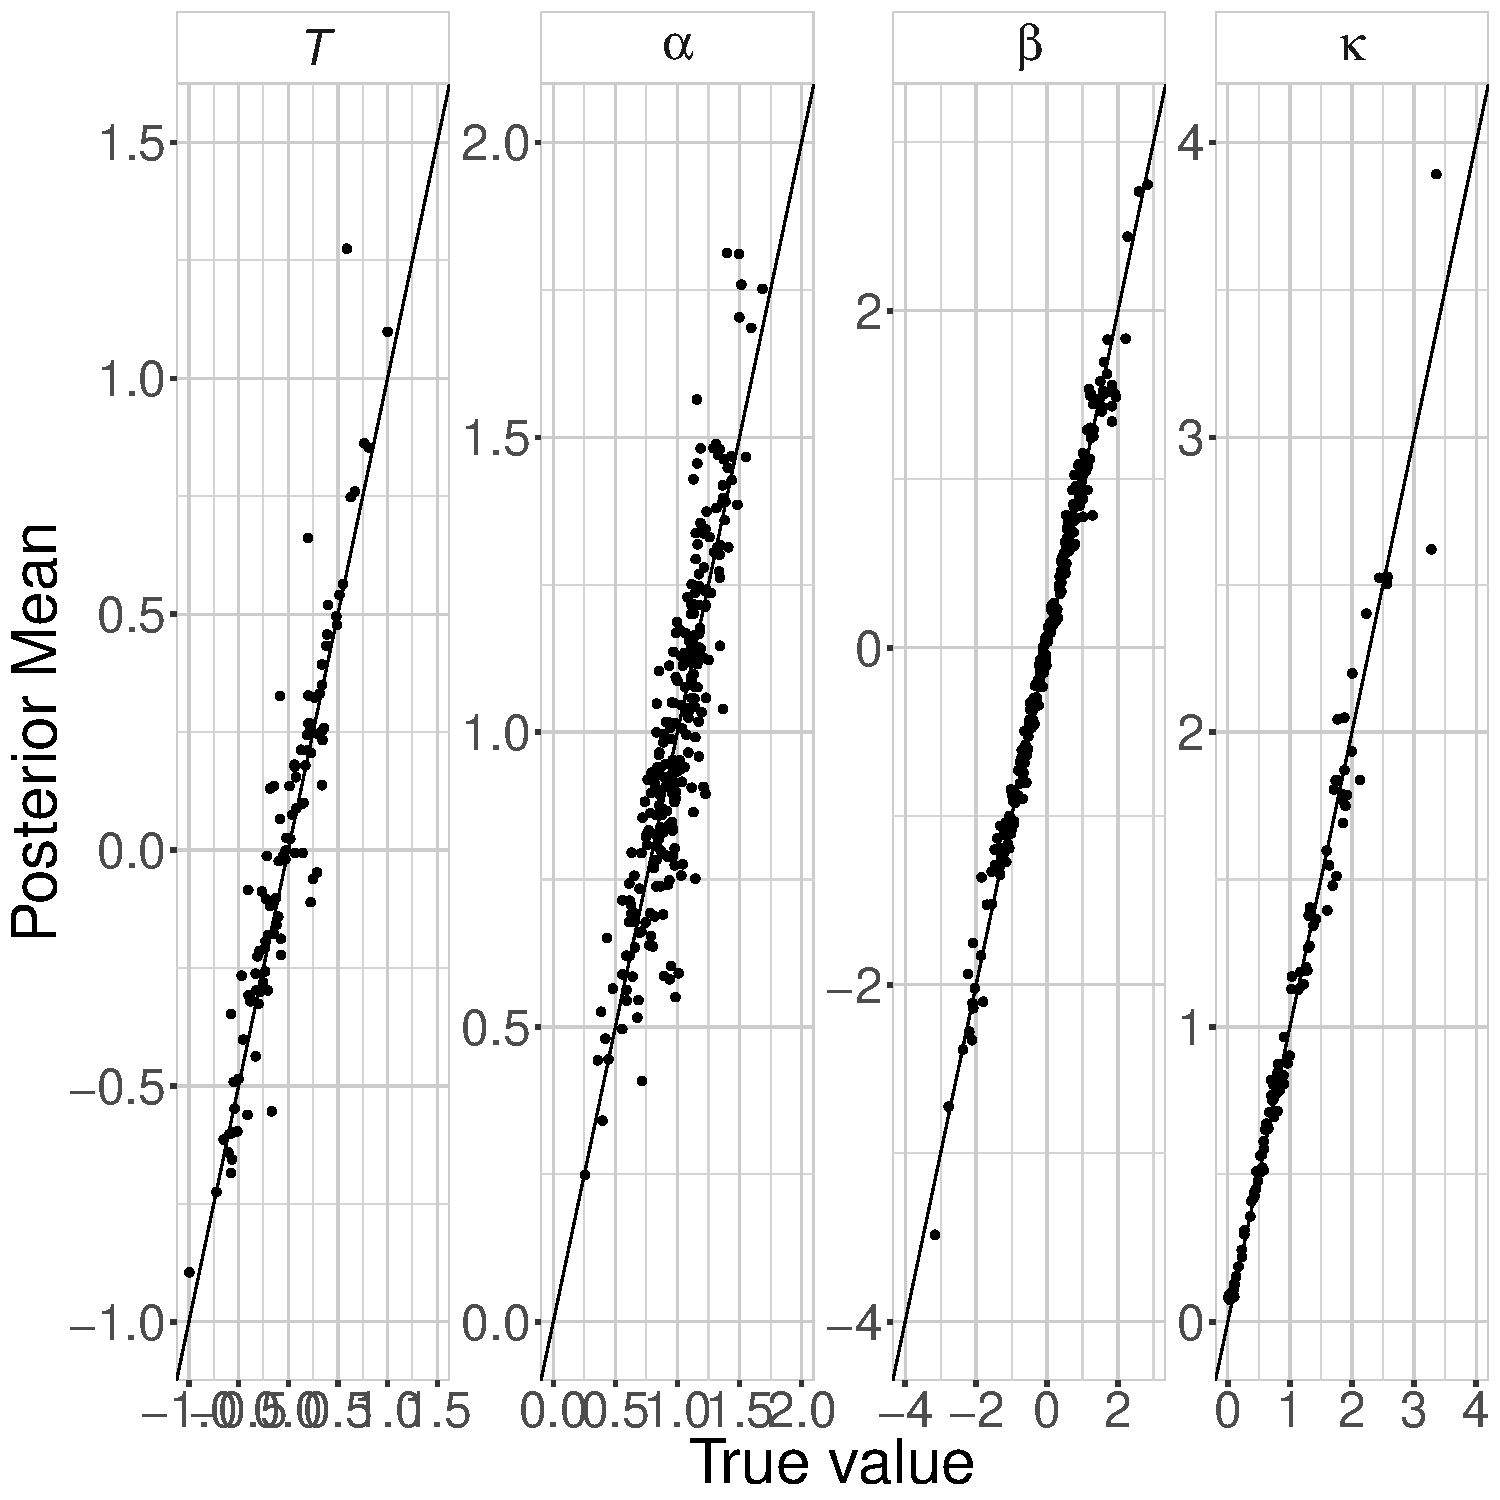
\includegraphics[width= \textwidth]{figures/parameterRecoveryModel1.pdf}
	\caption{Parameter recovery for the model displayed in Figure~\ref{model:LTRM}}
	\label{fig:parameterRecoveryM1}
\end{figure}

%\begin{figure}[!ht]
%	\centering
%	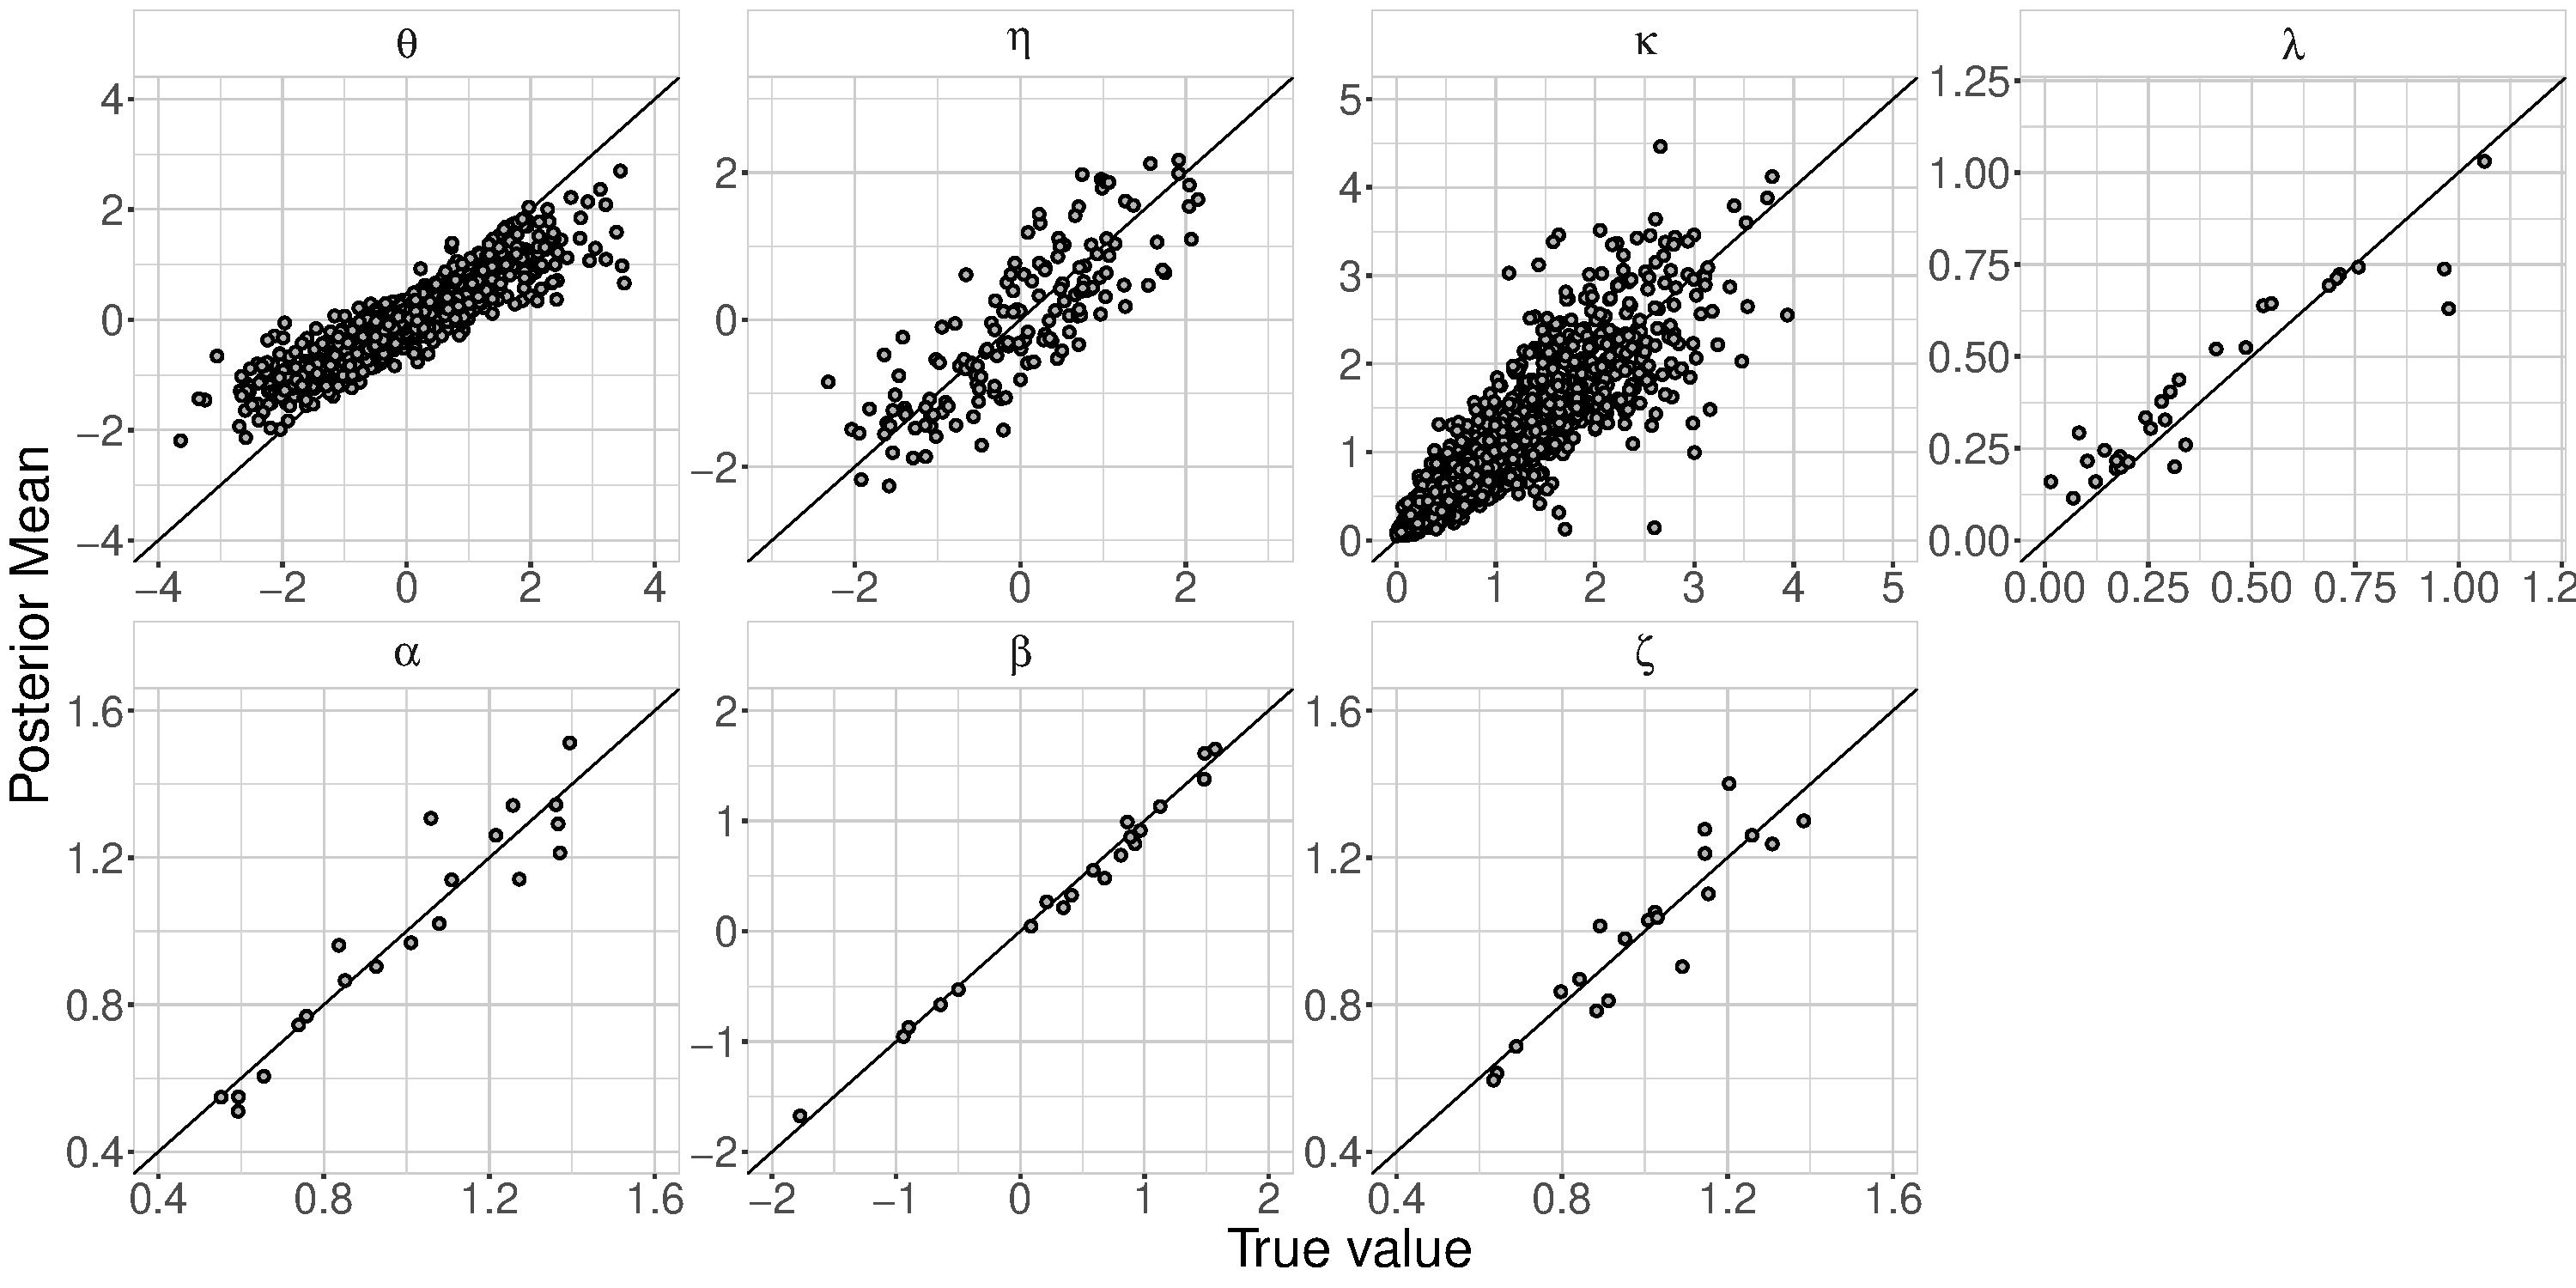
\includegraphics[width= \textwidth]{figures/parameterRecoveryModel2.pdf}
%	\caption{Parameter recovery for the model displayed in Figure~\ref{model:LTRM2}}
%	\label{fig:parameterRecoveryM2}
%\end{figure}

\end{document}

%\newpage
%
%
%personen/ raters zijn gebiased. Kan niet alleen eigenschappen van de gedetineerden halen maar ook die van de raters.
%
%Covariaat voor e.g., hulpverleners versus psychiaters. Meerdere groepen raters (fixed effect).
%
%Hierachisch niveau over patienten.
%
%Covariaat voor groepen gedetineerden (fixed effect misdrijf).
%Ofwel order restrictie voor deze groepen.
%
%Missing values?
%
%Hoe combineren we verschillende schalen van items?
%
%kaart van hoe ontwikkelt zich dit over de tijd (zie figuur in proposal)
%
%TODO: change model in NWO proposal to mimic SDT approach.
